\documentclass{article}

\usepackage{graphicx}
\usepackage{calc}
\usepackage{amsmath}
\usepackage[margin=1.0in]{geometry}
\usepackage{amsmath}
\usepackage[dvipsnames]{xcolor}
\usepackage{fancyhdr}
\usepackage{svg} 
\usepackage{listings}
\usepackage[final]{pdfpages}
\usepackage[parfill]{parskip}

\pagestyle{fancy}
\fancyhf{}
\rhead{Logan Torres}
\chead{}
\lhead{}
\rfoot{Page \thepage}
\linespread{1.5}

\begin{document}

\begin{center}
\huge\textbf{Capillary Migration of Large Confined drops in Super-hydrophobic Wedges}
\end{center} 

\begin{center}
\large Notes

\Large Logan Torres

\large April 2017
\end{center}

\noindent When confined within an interior corner, drops and bubbles
migrate to regions of minimum energy by the combined effects of surface tension,
surface wetting, and corner geometry. Such capillary phenomena are exploited for
passive phase separation operations in micro-fluidic devices on earth and macro-
fluidic devices aboard spacecraft. Our study focuses on the migration of large
inertial-capillary drops confined between two planar super-hydrophobic surfaces. In
our experiments, the near weightless environment of a drop tower produces Bo $\ll$ 1
for drop volumes $O$(10mL) with migration velocities up to 10 cm/s. We observe
transient behavior as a function of drop volume, wedge angle, initial
confinement, and fluid properties including contact angle. We then further demonstrate
how the experiment method may be employed as a large horizontal quiescent
droplet generator for studies ranging from inertial non-wetting moving contact line
investigations to large geyser-free horizontal drop impacts.

\hspace*{200pt}

\hrule
\section*{Introduction}
Surface tension, wetting characteristics, and geometric constraints can be used to control fluids in the limit of \textit{Bo} $\ll$ 1, as found in the weightless environments of deep space or in the micro-scale systems of inkjet printers, lab-on-a-chip systems, or other small devices.  In such a regime, pressure variations proportional to the mean curvature and surface tension by the Laplace Equation $\Delta P = \sigma \mathcal{K} $ are present and can constitute a sufficiently large pressure gradient when either the mean curvature $\mathcal{K}$ or surface tension value $\sigma$ varies across the fluid body. Such pressure induced flows can be controlled by gradients in temperature, introduction of surfactants, induced electro-wetting, geometric configurations, or combinations of these effects. The control of this capillary pressure by geometrical constraints poses an interesting study, as the passive nature of these systems is highly desirable. 

Creation and/or control of volumes of fluids such a droplets and bubbles are often the focus of said research. Immersed liquids in lab-on-a-chip devices, which are driven through micro-channels, exploit the enhanced effects of surface tension to generate precise volumes of reactants for controlled reactions and prodction of drugs mixtures. Dangla \textit{et al.} \cite{Dangla2013} proposed a passive confinement gradient for micro-fluidic droplet generation by exploiting the hydrodynamic instability of a immersed flow encountering a step change in a channel which is accompanied with nozzled upper and lower channel walls. Their research demonstrated the independence of droplet volume on the channel flow rate or fluid properties such that only geometrical changes were required for change in volume, a key benefit over other methods which are highly flow and fluid property dependent. For space systems, the contamination of fluid systems by bubbles can pose a dangerous challenge, as bouyancy effects are absent. Recently, methods for bubble coelences or removal from such fluids systems have been demonstrated by Jenson \textit{et al.} \cite{Jenson2014} through passive capillary migration of bubbles in conduits. This simple in design but complex in analysis system poses an advantage to high pressure system alternatives for its passive, reliable nature which is desired for long duration space missions. 

Apart from direct engineering investigations, analytical models to describe the dyanmic of droplets moving and orienting in wedge like geometries poses an interesting problem to solve. Reyssat \cite{Reyssat2014} pursued an analytical model for wetting droplets migrating into a wedge as well as non-wetting bubbles migrating out. Under a visco-capillary dominate regime, droplets and bubbles exhibit equivilent power law transient dyanmics as they migrate from their intial location. For droplets with contact angles satisfying the Concus-finn wetting condition \cite{Concus1998}, there is bulk migration of the droplet towards the wedge vertex where, once in contact, the volume will spread indefinitely. For contact angles greater the Concus-Finn wetting condition, the inverse problem is found which is also accompanied with a spherical equilibrium shape for drops and bubbles. Xu \textit{et al.} \cite{Xu2016} investigated the the equilibrium shapes for wedges oriented vertically with respect to gravity with controlled wettability by electro-wettting. 
   

\section*{Investigations}
\subsection*{Experimental}
The for-going confinement experiments were conducted under the micro-gravity environment of the Dryden Drop Tower located at Portland State University, which experiences gravity on the order \textit{O}($10^{-4}$) m/s$^2$ corresponding to the relevant non-dimensional parameter \textit{Bo} $\approx 10^{-4}$ for a free fall time of $t_d = 2.1$ s. Due to this near weightless environment, test volumes range up to \textit{O}($10$) mL. Super-hydrophobic surfaces of $\theta_{eq} = 151 \pm 5^{\circ}$ consist of a sheet of fine-grit sandpaper coated with an aerosol PTFE spray adhered to a flat, rigid acrylic plate. Data is acquired from high definition video taken from commercial camera system \cite{Camera} mounted to a drop tower test rig, and later post-processed using image processing software \cite{Software2004}.

\begin{figure}
	\centering
	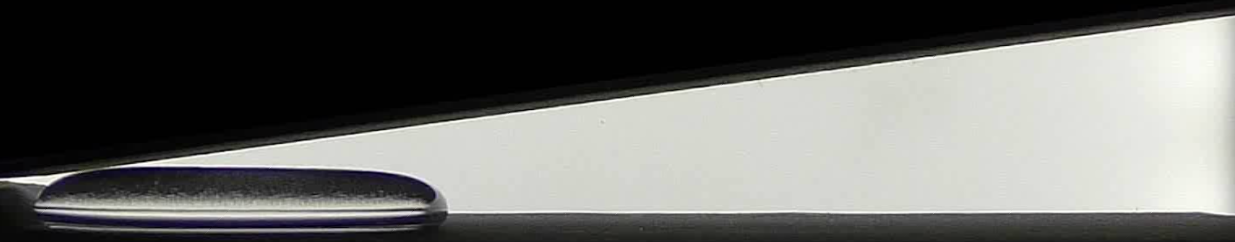
\includegraphics[scale=0.4]{Figures/initialcondition}
	\caption{}
	\label{fig:initial}
\end{figure}

Experiments conducted in the drop tower start with the volume of fluid resting under gravity on a horizontal, hydrophobic surface. A similar surface is held above and just slightly in contact with the droplet as depicted by Fig. (\ref{fig:initial}). Following the release of the experiment and a short re-orientation period, the trailing and leading edge menisci initial locations, identified in Fig. 2 as $X_{to}$ and $X_{lo}$ respectively, are measured by the known geometry of the system. The droplet location is then tracked using image processing software (Spotlight-16) by the trailing edge $X_t$.

\begin{figure}[h]
	
	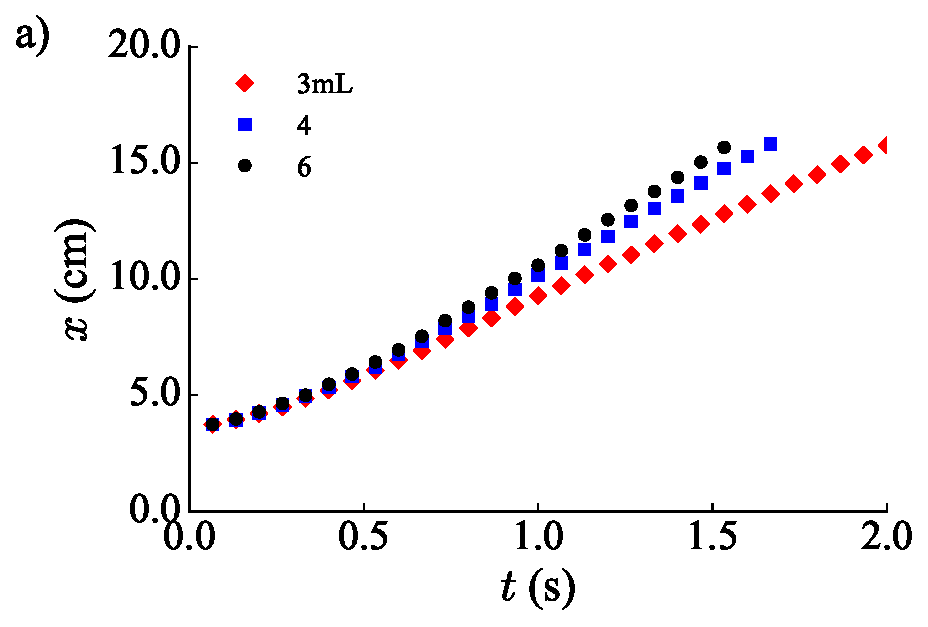
\includegraphics[scale=0.5]{Figures/VaryingVolume}
	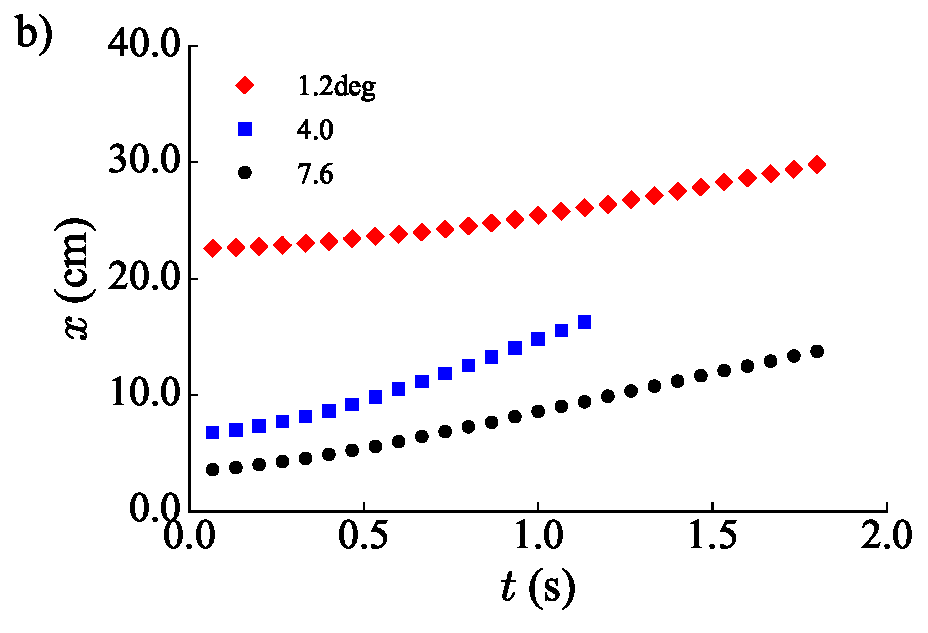
\includegraphics[scale=0.5]{Figures/VaryingAngle}
	\caption{a) 7.6$^\circ$ b) 3mL}
	\label{fig:Plot1}
\end{figure}

\subsection*{Analytical}
\subsubsection*{Pressure}

For the geometry above, we look to find an expression for the pressure difference encountered across the inside of the droplet. To reduce complexity, we find expressions for the radii of curvature for the advancing $r_2$ and receding $r_1$ menisci in terms of the corner half heights $h_2$ and $h_1$, given by
$
\frac{h_1}{r_1} = - \cos(\theta_1 - \alpha)
$
and 
$
\frac{h_2}{r_2} = -\cos(\theta_2 + \alpha)
$
where $\alpha$ is the coner half angle and $\theta_1$ and $\theta_2$ are the contact angles for the receding and advancing edges respectively. We note that $\theta_1$ and $\theta_2$ are bounded by $\theta_{advancing}$ and $\theta_{receding}$. Laplace's Law may be used to find the pressure difference across the convex interfaces 1 and 2 and are given by 

\begin{equation}
	\label{eq:generalpressure}
P_{io} - P_i = -\sigma \Big( \frac{1}{r_i} + \frac{1}{r_{io}} \Big) 
\end{equation} 

\noindent where $P_{io}$ is the ambient pressure, $P_i$ is the internal pressure of the droplet, $r_i$ is the radius of the interface, and $r_{io}$ is the out of plain radius of curvature, all evaluated at location $i$. Note the negative value in front of the fraction accounts for the convex profile of each menisci. Evaluating Eq. (\ref{eq:generalpressure}) at both interfaces identified in Fig. (\ref{fig:schematic}) and taking the difference noting that the external pressure field and out of plane radius of curvature is the same for both interfaces, we find the pressure difference between interface 2 and 1 as follows 

\begin{equation}
\label{eq:pressurediff}
P_1 - P_2 = \sigma \Big(  \frac{\cos(\theta_2 + \alpha)}{h_2} -\frac{\cos(\theta_1 + \alpha)}{h_1} \Big)
\end{equation}
          
\noindent Taking note the relationship between the half widths of each interface we find that $h_1 < h_2$. Furthermore the contact angle for each edge is greater than $\pi/2$, $\theta_{1,2} \gg \pi/2$, and therefore $\cos(\theta_{1,2} \pm \alpha) < 0$. We now resolve that the pressure inside interface 1 is greater than the pressure inside face 2, $P_1 - P_2 > 0$, resulting in spontaneous migration away from the apex.

A second pressure term is present and acts perpendicular to the top and bottom surfaces with a contribution proportional to the sin of the half angle in the direction of interface 2. Averaging the pressure inside both mensici, $
P_{ave} = P_o -  \frac{\sigma}{2} \Big(  \frac{\cos(\theta_2 + \alpha)}{h_2} +\frac{\cos(\theta_1 + \alpha)}{h_1} \Big)$ , and evaluating a force balance on each surface we get 
$$
P_{ave} - P_o =  \frac{\sigma}{2} \Big(  \frac{\cos(\theta_2 + \alpha)}{h_2} +\frac{\cos(\theta_1 + \alpha)}{h_1} \Big)
$$

\begin{figure}
	\centering
	
\includegraphics[scale=0.65]{Figures/Schematic2}
	\caption{}
	\label{fig:schematic}
\end{figure}

\subsubsection*{Scaling}
The drop jump velocity is estimated analytically in the large puddle volume limit by assuming a
sufficiently non-wetting puddle of cylindrical disk shape with radius $R_1$ and height $H$. We ignore viscous
losses due to shear, roll-up, receding contact line motion, and air drag. We assume the drop ultimately
achieves a spherical configuration of radius $R_2 = R_d$ and that no satellite drops are formed. Non-spherical
distortions of the drop during the jump are eventually damped by viscous forces which are also ignored.
These idealized initial and final states are depicted schematically in Fig. 11b and c.

Using the notation of Fig. 11b and c, the surface energies for liquid-solid ($ls$), gas-liquid ($gl$), and solid-
gas ($sg$) for cylindrical disk and spherical shapes are $SE_1 = [(\sigma A)_{ls} + (\sigma A)_{gl} + (\sigma A)_{sg} ]_1$ and $SE_2 = [(\sigma A)_{gl} +
(\sigma A)_{sg} ]_2$ , respectively. From Young’s equation we have $\sigma_{sl} - \sigma_{sg} = \sigma_{gl} cos\theta$, where $R_1 = R_p = (V_d /\pi H)^{1/2}$ , $R_2
= R_d = (3V_d /4\pi)^{1/3}$ , and $H \approx 2(\sigma/\rho g)^{1/2}$ . From $KE = SE_1 - SE_2$ we find

\begin{equation}
{U} = \frac{\sigma g}{\rho}^{1/4} \Big[ -2\cos\theta + 2\big(\frac{\pi H^3}{V_d}\big)^{1/2} - 6^{2/3}\big(\frac{\pi H^3}{V_d}\big)^{1/3}\Big]^{1/2} \equiv \Big(\frac{\sigma \tilde{We}_j}{\rho R_d}\Big)^{1/2}
\end{equation}

In the large puddle limit $(\pi H^3 /V_d)^{1/3} \ll 1$, and for $\pi/2 \leq \theta \leq \pi$, eq. (5) reduces to

\begin{equation}
{U} = \Big(\frac{\sigma g}{\rho}\Big)^{1/4} \big(-2\cos\theta\big)^{1/2}
\end{equation}

when $\theta = \pi$ the maximum puddle jump limit is found to be 

\begin{equation}\tilde{U} \approx \Big(\frac{4\sigma g}{\rho}\Big)^{1/4}
\end{equation}

Identifying an inscribed location $L_R \approx R/\sin\alpha$ where $R
= R_{sphere} = (3V_d /4\pi)^{1/3}$ and initial confined location $x_o = H/2\sin\alpha$ where $H \approx 2(\sigma/\rho g)^{1/2}$ along with the the scale velocity $\tilde{U}$, we find the ejection time $
t_{jw} = \frac{L_r-x_o}{U} \approx \frac{\frac{3V}{4\pi}^{1/3} - \frac{H}{2}}{\tilde{U}\sin\alpha}
$. Expanding velocity term we find 


\begin{equation}
t_{jw} = \frac{\big(\frac{3V}{4\pi}\big)^{1/3}\big(\frac{\rho}{\sigma g}\big)^{1/4}}{\sin\alpha} \frac{\Big[1 - 6^{1/3}(\frac{\pi H^3}{V})^{1/3}\Big]}{\Big[-2\cos\theta + 2\frac{\pi H^3}{V}^{1/2}- 6^{2/3}(\frac{\pi H^3}{V})^{1/3}\Big]}
\end{equation} 
Under the small volume approximation $\frac{\pi H^3}{V}^{1/3} \ll 1$

\begin{equation}
t_{jw} = \Big(\frac{3V}{4\pi}\Big)^{1/3}\Big(\frac{\rho}{\sigma g}\Big)^{1/4}\frac{1}{-2\cos\theta\sin\alpha} 
\end{equation} 

\begin{figure}
	\centering
	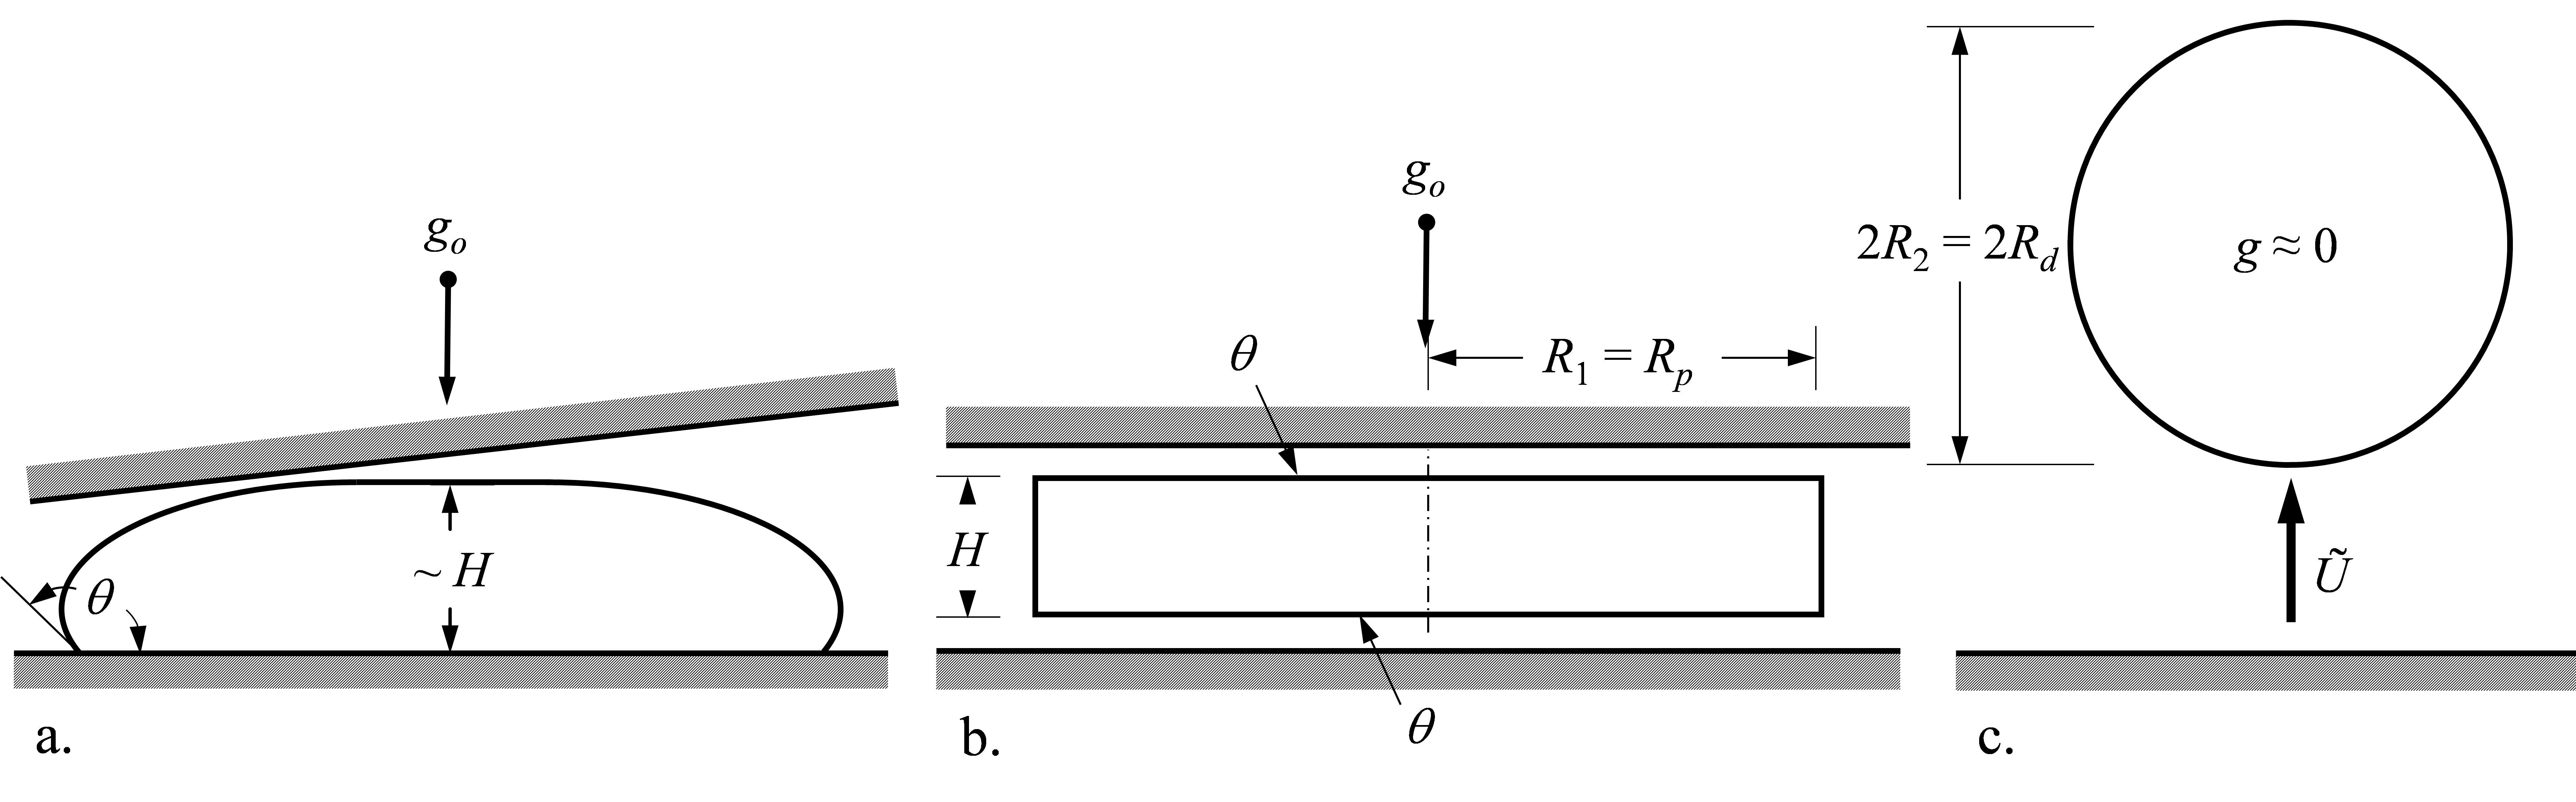
\includegraphics[scale=0.13]{Figures/PuddleJump}
	\caption{Given}
\end{figure}

\subsection*{Volume} 

The wedge droplet can be constructed from two geometries: (1) an internal sliced column and (2) a variable internal radius torus. Volume (1) is easily solved in terms of its diameter, $2R$, which is represented by the perpendicular distance between $h_1$ and $h_2$ (see Fig. 1) given by

\begin{equation} 
V_{inner} = \pi R^2 (h_1 + h_2)
\end{equation}

Volume (2) is more challenging. The complexity of the problem is resolved by taking an average of two outer-half torii of radius $h_1$ and $h_2$. The area of a circular segment is given by

\begin{equation}A_{seg} = r^2 \Big( \frac{2\beta_{1,2} - \sin2 \beta_{1,2}}{2} \Big)
\end{equation}

where $\beta_{1,2} = \theta_{1,2} \pm \alpha - \pi/2$. This area is revolved around the droplet average center indentified in Fig. (1) to compute the volume.

\begin{equation} 
V_{seg} = 2\pi(R+\Delta r)r^2 \Big( \frac{2\beta_{1,2} - \sin2 \beta_{1,2}}{2} \Big) 
\end{equation}

where $\Delta r = r \frac{4\sin^3\beta}{6\beta - 3\sin2\beta} - r\cos\beta$ is the distance from the segment planar face to the segment centroid. 

\begin{equation}V_{seg} = 2\pi R r^2 \Big( \frac{2\beta - \sin2 \beta}{2} \Big) + 2\pi r^3 \Big( \frac{2\beta - \sin2 \beta}{2} \Big)\frac{4\sin^3\beta}{6\beta - 3\sin2\beta} - 2\pi r^3 \Big( \frac{2\beta_{1,2} - \sin2 \beta_{1,2}}{2} \Big)\cos\beta
\end{equation}

\begin{equation}
V_{seg} = 2\pi \Big(Rr^2 - r^3\cos\beta\Big)  \Big( \frac{2\beta - \sin2 \beta}{2} \Big) + 2\pi r^3 \Big( \frac{4\sin^3\beta}{6} \Big)
\end{equation}


Using the relationships of eq. (1) and (2) along with $\beta = \beta(\theta,\alpha)$ from eq. (7) $r = h/\sin\beta$ we substitue and resolve

\begin{equation}
V_{seg} = \frac{4\pi}{3} h^3 + 2\pi \Big(Rh^2\sin\beta - h^3\cos\beta\Big)  \Big( \frac{2\beta - \sin2 \beta}{2\sin^3\beta} \Big)
\end{equation}

which matches a test drawing of a segmented toriod in SolidWorks.

We want to determine the pressure at each location of the droplet as a function of time x(t). 



$\beta$ is a function of the contact angle and the corner half angle, which we assume is different the front and back meniscii. Therefore, to find the estimated volume of the outter toroid, we average eq. (11) using the given heights and $\beta$s for each menscii respectively.

$$\phi= \frac{2\beta - \sin2 \beta}{2\sin^3\beta}$$

\begin{equation}
V_{seg_{ave}} = \frac{2\pi}{3}(h_1^2 + h_2^2) + \pi\Big(R\big(h_1^2\sin\beta_1 \phi_1+h_2^2\sin\beta_2 \phi_2\big) - \big(h_1^3\cos\beta_1\ \big)\Big)
\end{equation} 

\pagebreak

\section*{Appendix}
 

\begin{equation}
\frac{h_1}{r_1} = \sin(\theta_1 - \alpha - \frac{\pi}{2}) = - \cos(\theta_1 - \alpha)
\end{equation}

\begin{equation}
\frac{h_2}{r_2} = sin(\theta_2 + \alpha - \frac{\pi}{2}) = -\cos(\theta_2 + \alpha
\end{equation}

\begin{equation}
P_o - P_1 = -\sigma \Big( \frac{1}{r_1} + \frac{1}{r_3} \Big) = \sigma \Big( \frac{\cos(\theta_1 - \alpha)}{h_1} - \frac{1}{r_3} \Big)
\end{equation} 

\begin{equation}
P_o - P_2 = -\sigma \Big( \frac{1}{r_2} + \frac{1}{r_3} \Big) = \sigma \Big( \frac{\cos(\theta_2 + \alpha)}{h_2} - \frac{1}{r_3} \Big)
\end{equation}

\begin{equation}
(P_o - P_2) - (P_o - P_1) = P_1 - P_2 = \frac{\sigma \cos(\theta_2 + \alpha)}{h_2} - \frac{\sigma \cos(\theta_1 + \alpha)}{h_1}
\end{equation}
\begin{equation}
P_1 - P_2 = \sigma \Big(  \frac{\cos(\theta_2 + \alpha)}{h_2} -\frac{\cos(\theta_1 + \alpha)}{h_1} \Big)
\end{equation}

\pagebreak

\bibliography{mycollection} 
\bibliographystyle{ieeetr}

\end{document}

